\documentclass{beamer}
\usetheme{metropolis}           % Use metropolis theme
\usepackage{outlines}
\usepackage{listings}
%\usepackage{minted}
%\usepackage{pygmentiz}


\title{Introducción y Conceptos básicos de bases de datos}
\date{\today}
\author{Alex Di Genova}
\institute{Universidad de O'higgins}
\begin{document}
  \maketitle
  
  
  
  \begin{frame}{Outline}
  \tableofcontents
\end{frame}

\section{Bienvenida curso de Bases de datos}
  \begin{frame}{Presentación}     
   % \begin{itemize}
\only<1>{
  Alex Di Genova
    \begin{outline}
    \1 2003--2008 Ingeniero en Bioinformática. 
    \1 2013-2017 Doctor en Sistemas Complejos.
    \1 2017-2021 Postdoctorado en algoritmos y cáncer (Francia).
    \1 2022 - Profesor Asistente UOH.
    \2 Di Genoma Lab 
    	\3 Combinamos el desarrollo de nuevos algoritmos, análisis de genomas y tecnologías ómicas de última generación para estudiar sistemas biológicos complejos.
    \end{outline}
   }
   
   \only<2>{
   \begin{figure}
  \centering
    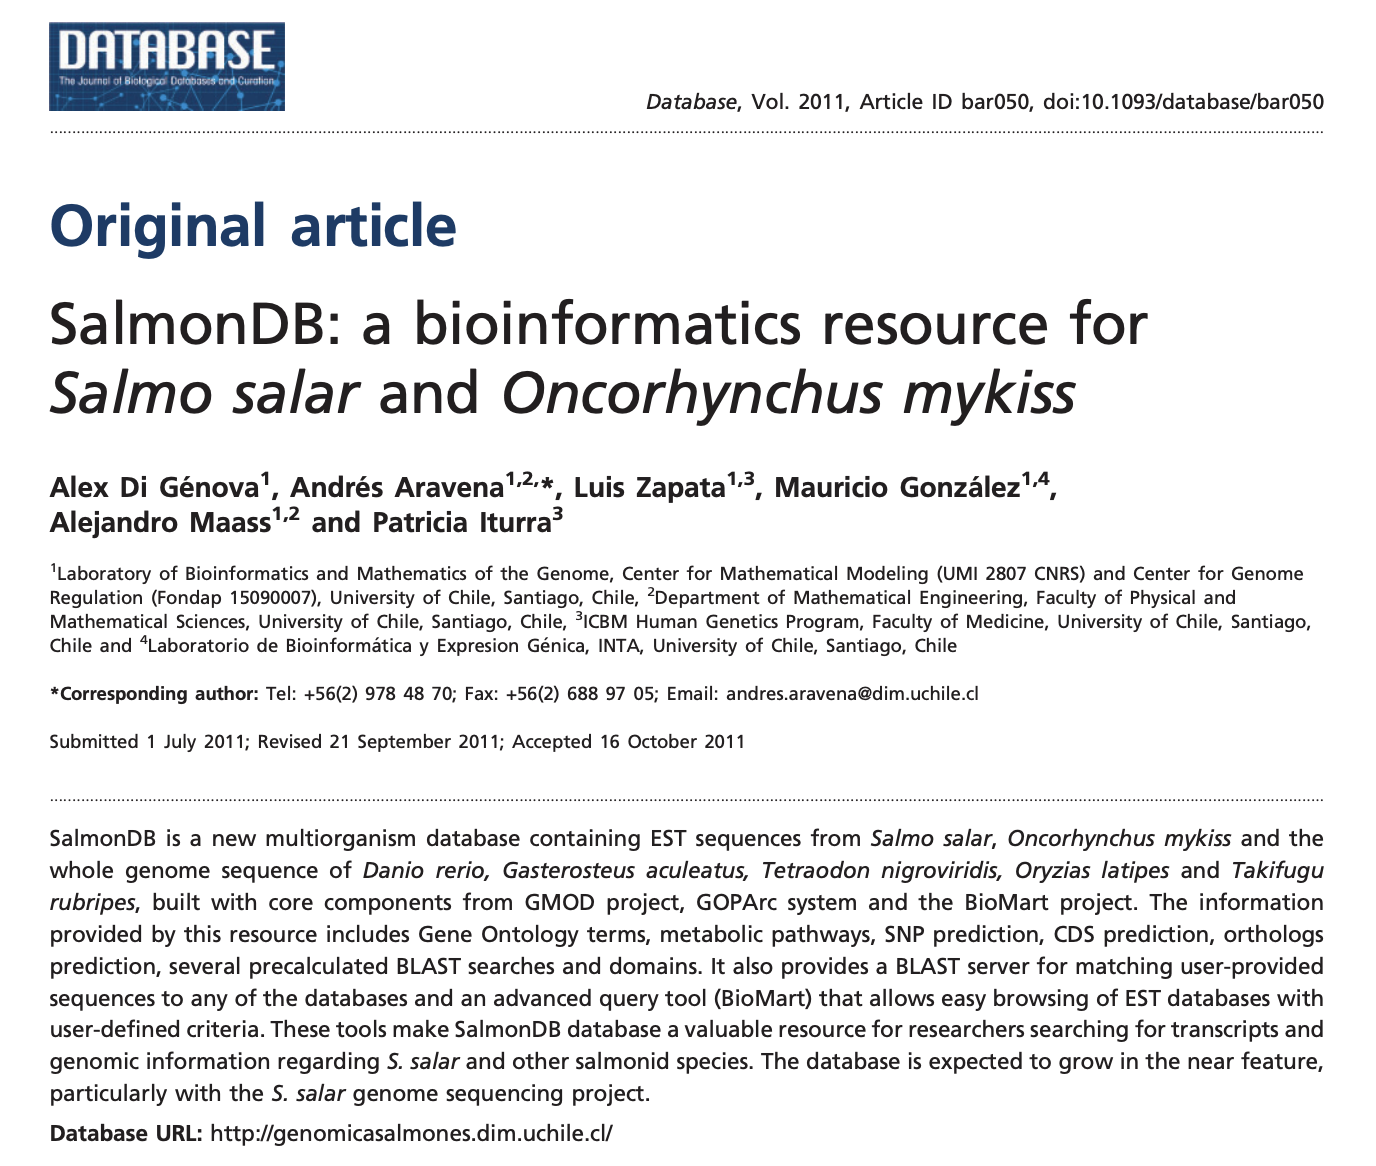
\includegraphics[scale=0.4]{img/salmondb.png}
 \end{figure}
   } 
   \only<3>{
   \centering
   \Large
   Alumnas y Alumnos
   }
  \end{frame}
 
  \section{Bases de datos}
 
 
 
 \begin{frame}{Qué es una base de datos?}
\begin{outline}
\1 Recopilación organizada de datos interrelacionados que
modelan algún aspecto del mundo real.
\1 Las bases de datos son el componente central de la mayoría
de las aplicaciones computacionales (Facebook, Instagram, \dots).
%\2
\end{outline}
 \end{frame}


 \begin{frame}{Cuando usamos una base de datos?}
 Usamos una base de datos, sí:
 \begin{outline}
 \1 Realizamos la inscripción de un curso en la universidad.
 \1 Realizamos una transferencia bancaria.
 \1 Realizamos compras online.
 \1 Utilizamos las redes sociales.
 \1 Utilizamos Spotify o Apple music.
 \1 Otros \dots
 \end{outline}
 \end{frame}
 
 \begin{frame}{Ejemplo de bases de datos}
 Crear una base de datos que modele el proceso de inscripción de cursos en una universidad
para realizar un seguimiento de los estudiantes y los cursos.

\uncover<2->{
Cosas que debemos almacenar:
\begin{outline}
	\1 Información de los estudiantes (Nombre, Apellido, edad, \dots )
	\1 Que cursos inscribieron los estudiantes (Nombre, semestre, calificación, \dots) 
\end{outline}
}
 \end{frame}
 
 \begin{frame}{Solución basada en archivos}
 
Almacenaremos nuestros datos de estudiantes y cursos utilizando archivos separados por tabulador, que serán manipulados con código propio. 

\uncover<2->{
Cosas que debemos hacer:
\begin{outline}
	\1 Para cada entidad crear un archivo (Estudiantes, Cursos, \dots )
	\1 Nuestro código debe soportar operaciones con los archivos y registros (leer, actualizar, buscar, \dots) 
\end{outline}
}

\uncover<3->{


 Creamos la base de datos usando los siguientes archivos:
 \tiny
\begin{columns}
\begin{column}{0.5\textwidth}

\begin{block}{Alumno}
\begin{tabular}{lcc}
    Nombre & Edad& Mail \\
\hline
    Alicia & 21 & alicia@gmail.com \\
    Bob & 22 & bob@gmail.com \\
    Carlos & 19 & carlos@gmail.com\\
    &  & \dots \\
\end{tabular}
\end{block}

 \end{column}
\begin{column}{0.5\textwidth}  %%<--- here
\begin{block}{Curso}
\begin{tabular}{lcc}
    Nombre & Semestre & Alumno \\
\hline
    BD & 1 & alicia \\
    Programación & 4 & bob \\
    Química & 1 & carlos\\
    BD & 1 & bob \\
    Programación & 4 & carlos \\
     &  & \dots \\
\end{tabular}
\end{block}

\end{column}
\end{columns}

}
 \end{frame}
 
 
 
 \begin{frame}[fragile]{Solución basada en archivos}
 Ejemplo:
 \begin{itemize}
\item Obtener los cursos realizados por alicia.
 \end{itemize}
 \rule{\textwidth}{1pt}
\begin{lstlisting}[language=Python]
file = open("Curso.txt")
for line in file:
 record = parse(line)
  if "alicia" == record[3]
   print record
   
# DB 1 alicia

\end{lstlisting}
\rule{\textwidth}{1pt}
\end{frame}
 
 
  \begin{frame}{Problemas de la solución basada en archivos}
%\begin{scriptsize}

  \begin{outline}
  \1 Integridad de los datos
  \2 Como nos aseguramos que el/la alumn@ es él mismo en el archivo de Cursos?
  \2 Qué pasa si alguien almacena el  campo semestre con una palabra (1$->$ primer)?
  \2 Como almacenamos múltiples alumnos en un curso?
  \uncover<2->{\1 Implementación
%  \2 Cómo podemos encontrar un registro en particular?
  \2 Cómo podemos actualizar un o un grupo de registros?
  \2 Qué pasa si ahora queremos crear una nueva aplicación que usa la misma base de datos?
  \2 Qué pasa si dos aplicaciones actualizan al mismo tiempo al archivo Curso.txt?}
  \uncover<3->{
  \1 Fiabilidad
  \2 ¿Qué pasa si la máquina falla mientras  estamos
actualizando un registro en alumno o Curso?
  \2 ¿Qué pasa si queremos replicar la base de datos en varias máquinas para tener alta disponibilidad?}
  \end{outline}
 % \end{scriptsize} 
  \end{frame}
 
  \begin{frame}{Sistema de administración de bases de datos (DBMS)}
    \only<1>{
  \begin{figure}
  \centering
    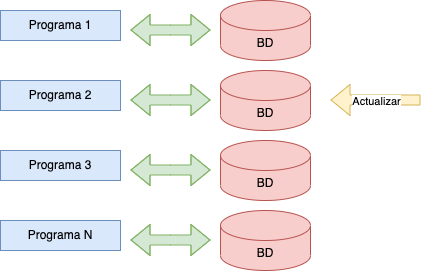
\includegraphics[scale=0.5]{img/file_app.png}
 \end{figure}
 \begin{outline}
 \1 Solución basada en archivos
 \2 Redundancia de código.
 \2 Redundancia de datos.
 \2Inconsistencia de datos.
 \end{outline}
}
 \only<2>{
  \begin{outline}
\1 Un DBMS es un software que permite a las aplicaciones
almacenar y analizar información en una base de datos.
 \1 Un DBMS de propósito general está diseñado para permitir la definición, creación, consultas, actualización y administración de bases de datos.
 \2 MySQL, PostgreSQL, Microsoft SQLServer,  Oracle, \textbf{SQLite}
 \3 Structured Query Language (SQL)
 \end{outline}
  \begin{figure}
  \centering
    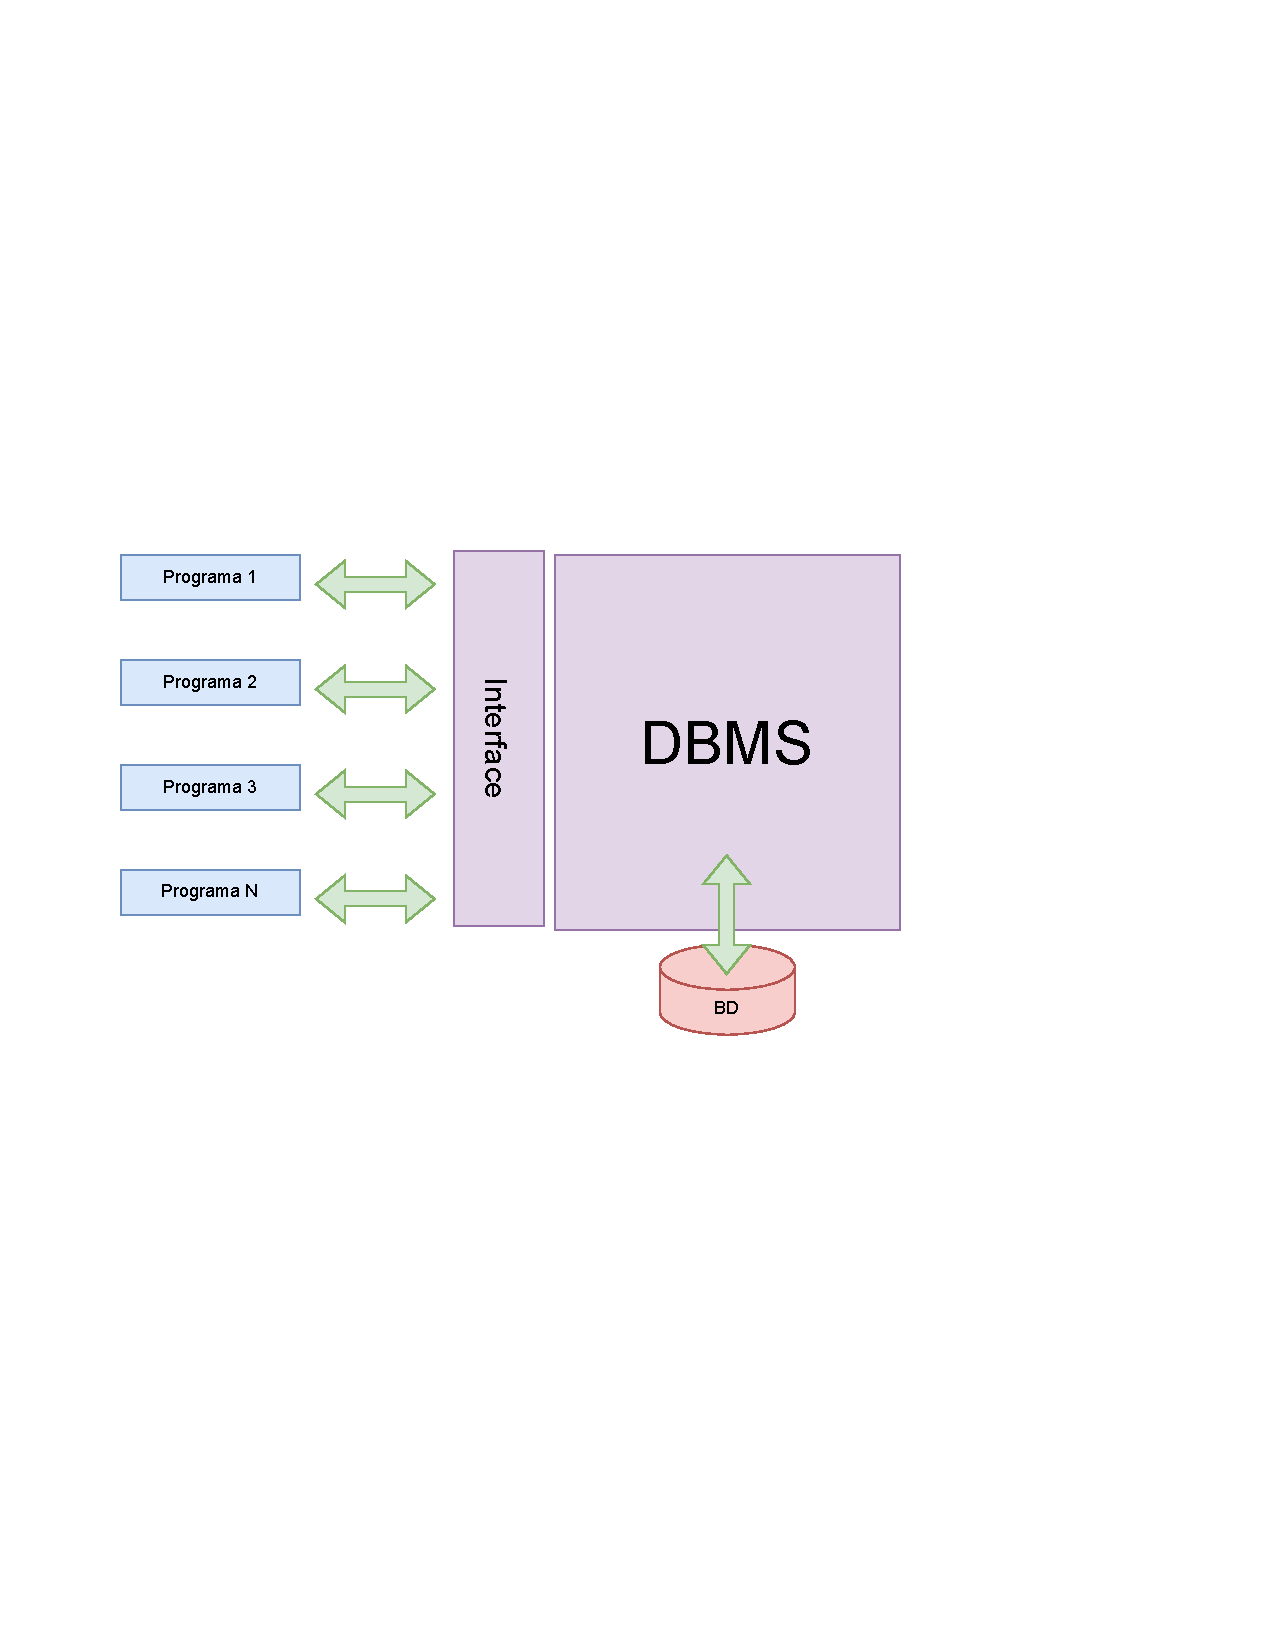
\includegraphics[scale=0.5]{img/file_systemdbms.pdf}
 \end{figure}
} 

  \end{frame} 
 
 
 
  \section{Planificación curso BD}
 \begin{frame}{Unidades}
  \only<1>{
    \begin{itemize}
    	\item 4 Unidades (14 semanas)
		\begin{itemize}
			\item Modelamiento de bases de datos (3 semanas)
			\item Modelo Relacional (4 semanas)
			\item Lenguaje de Consulta SQL (3 semanas) 
			\item Transacciones y Bases de datos no relacionales (4 semanas)
		\end{itemize}
	  \end{itemize}
}
 \only<2>{
Modelamiento de bases de datos 
\begin{itemize}
\item \emph{Cada \textbf{persona} puede habitar en solo una \textbf{vivienda} y estar registrada en solo un \textbf{municipio} pero pude ser propietaria de varias viviendas.} \dots
\item La \textbf{empresa} está organizada en \textbf{departamentos}. Cada uno tiene un nombre único, un número único y un empleado concreto que lo administra. Un departamento controla una cierta cantidad de \textbf{proyectos}, cada uno de los cuales tiene un nombre único, un número único y una sola ubicación.
\end{itemize}
}
\only<3>{
Esquema Relacional 
\begin{figure}
  \centering
    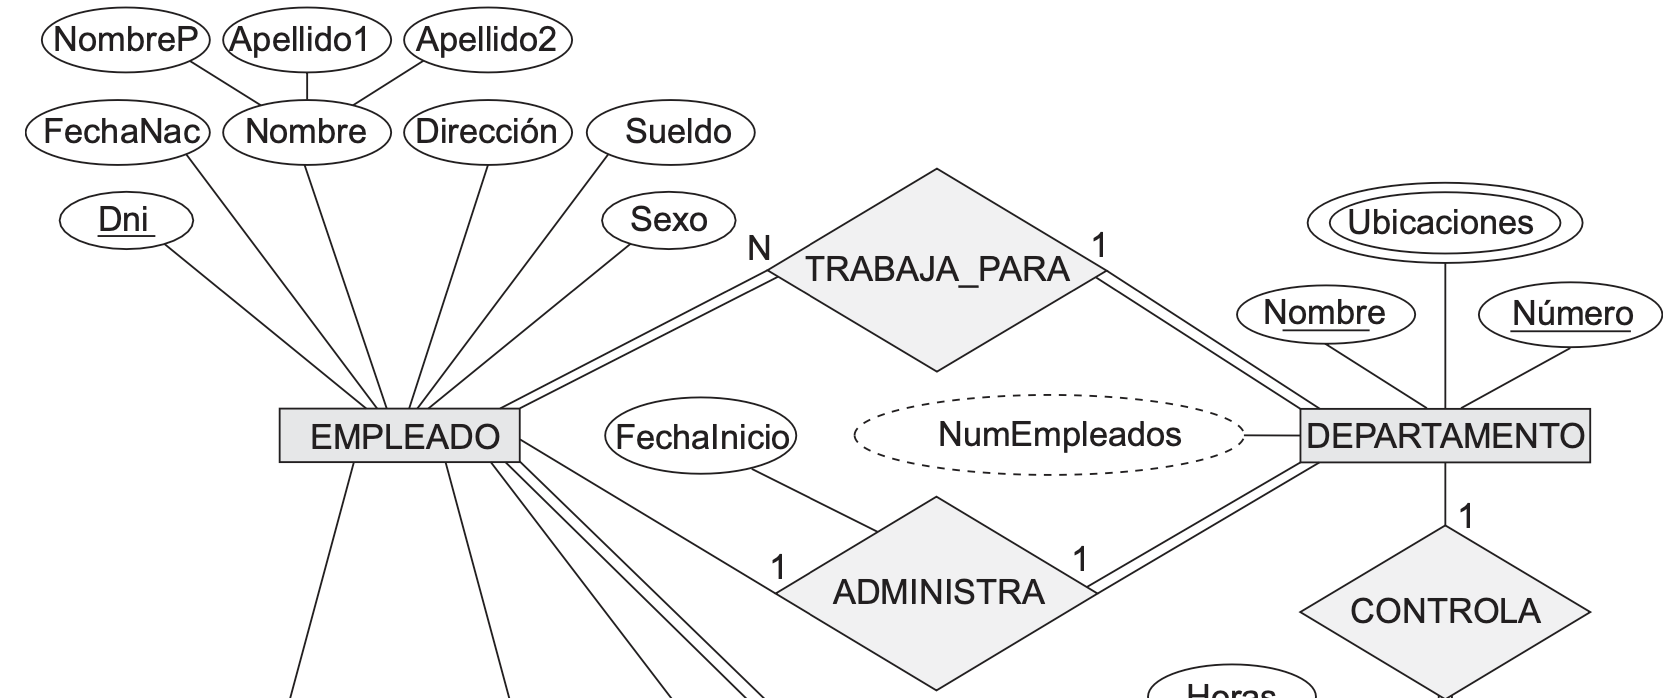
\includegraphics[scale=0.4]{img/er.png}
 \end{figure}
}
\only<4>{
Diagrama Entidad-Relacion (Modelo UML)
\begin{figure}
  \centering
    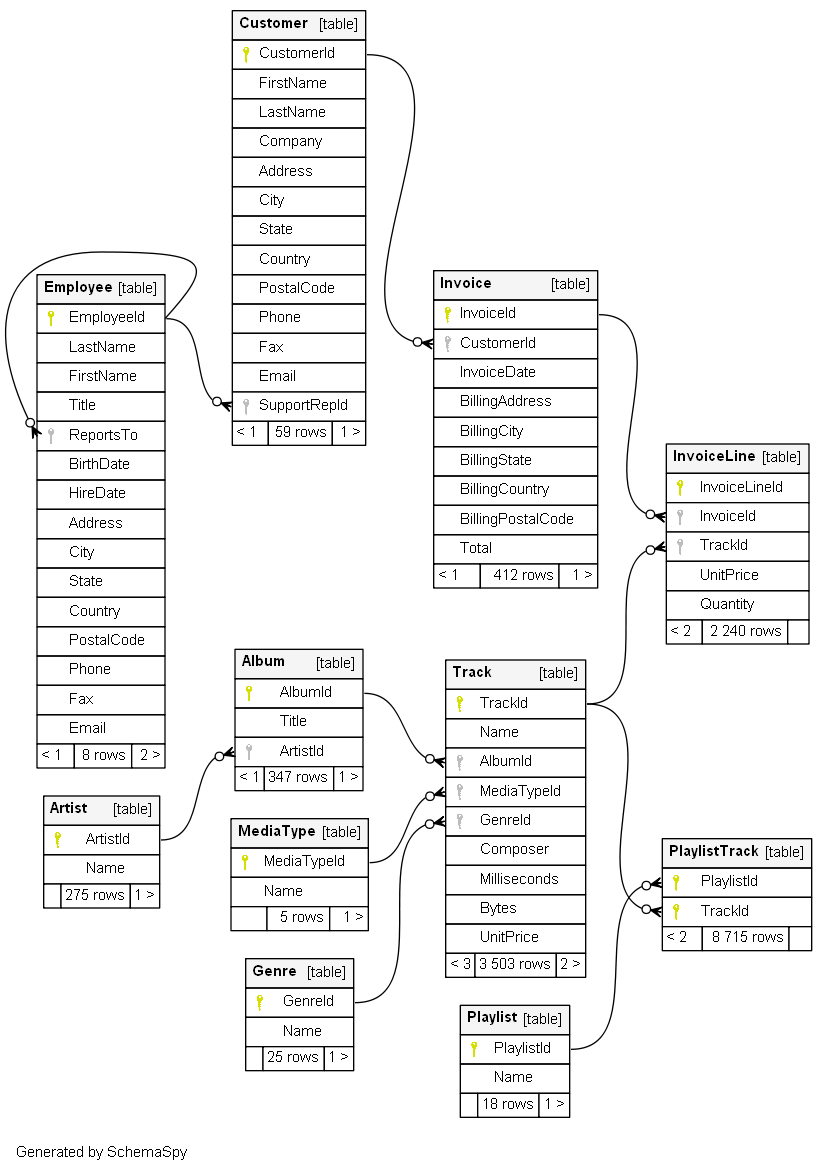
\includegraphics[scale=0.2]{img/db-uml.png}
 \end{figure}
}
\only<5>{

SQL (SQLite3)
\begin{figure}
  \centering
    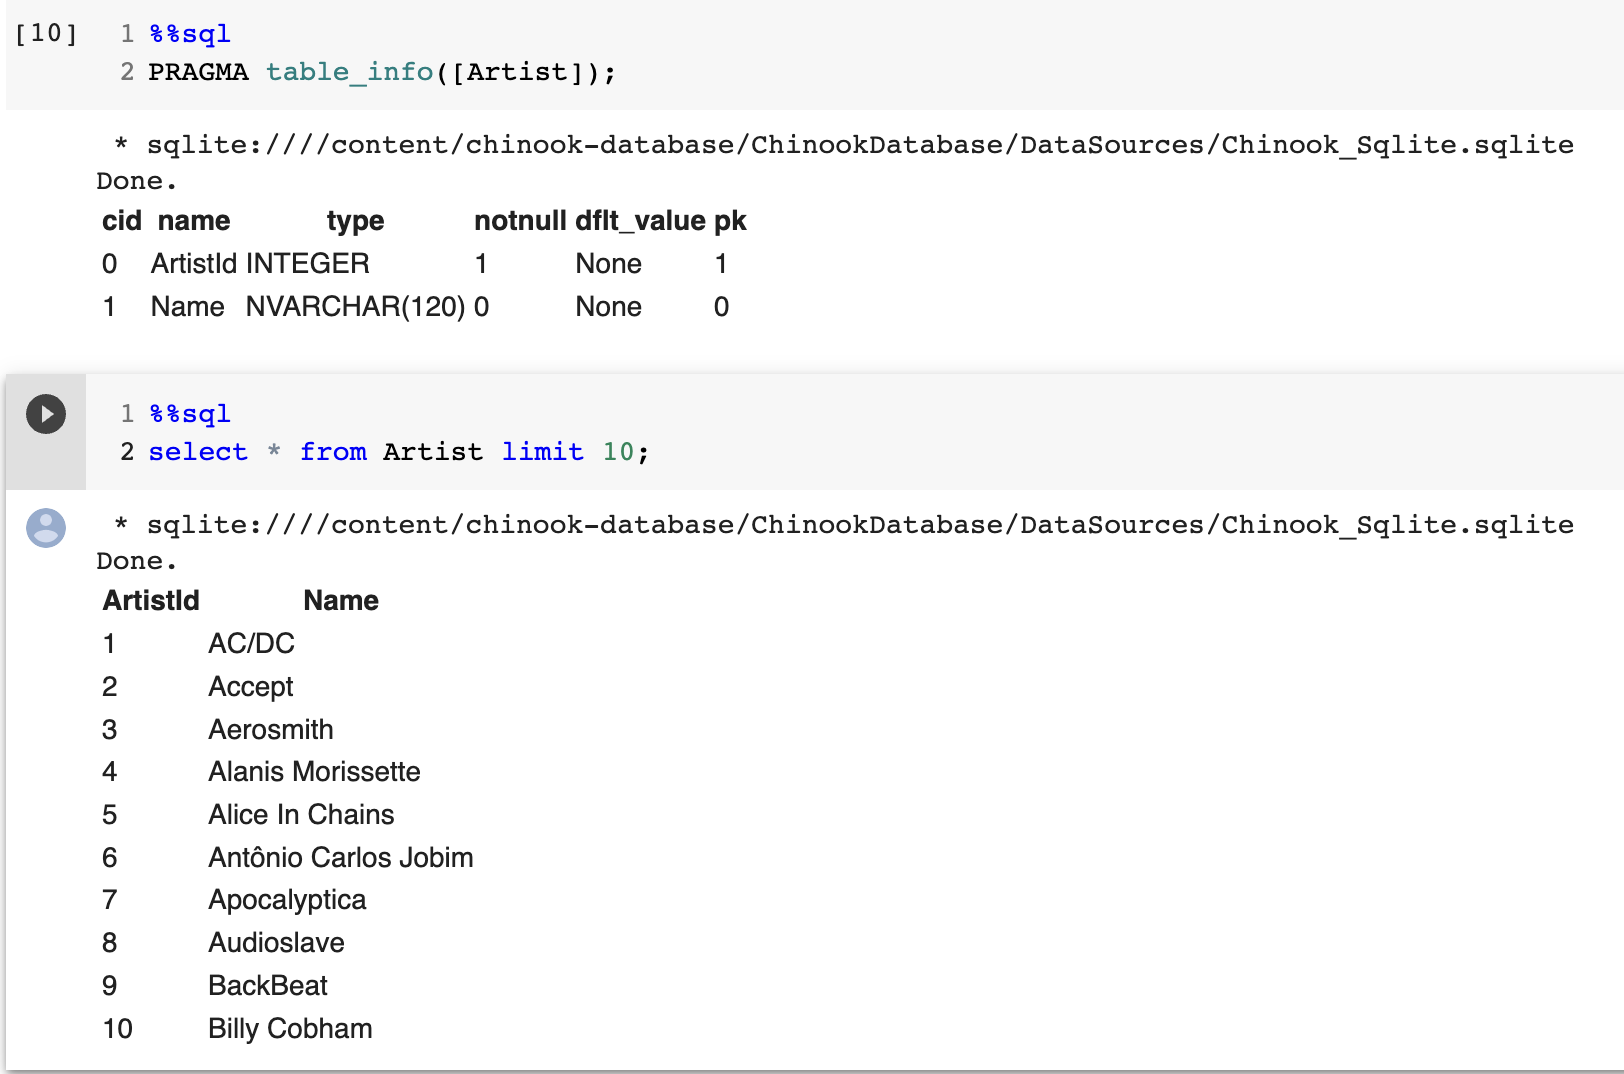
\includegraphics[scale=0.3]{img/sql-ex.png}
 \end{figure}
 
 GoogleColab -- \url{https://colab.research.google.com/}
 
  \href{https://www.youtube.com/watch?v=8VFYs3Ot_aA&t=115s}{Video descriptivo de GoogleColab}

}
\only<6>{
Transacciones
\begin{itemize}
\item Atomicidad
\item Conservación de la consistencia.
\item Aislamiento
\item Durabilidad
\end{itemize}
	\begin{figure}
  \centering
    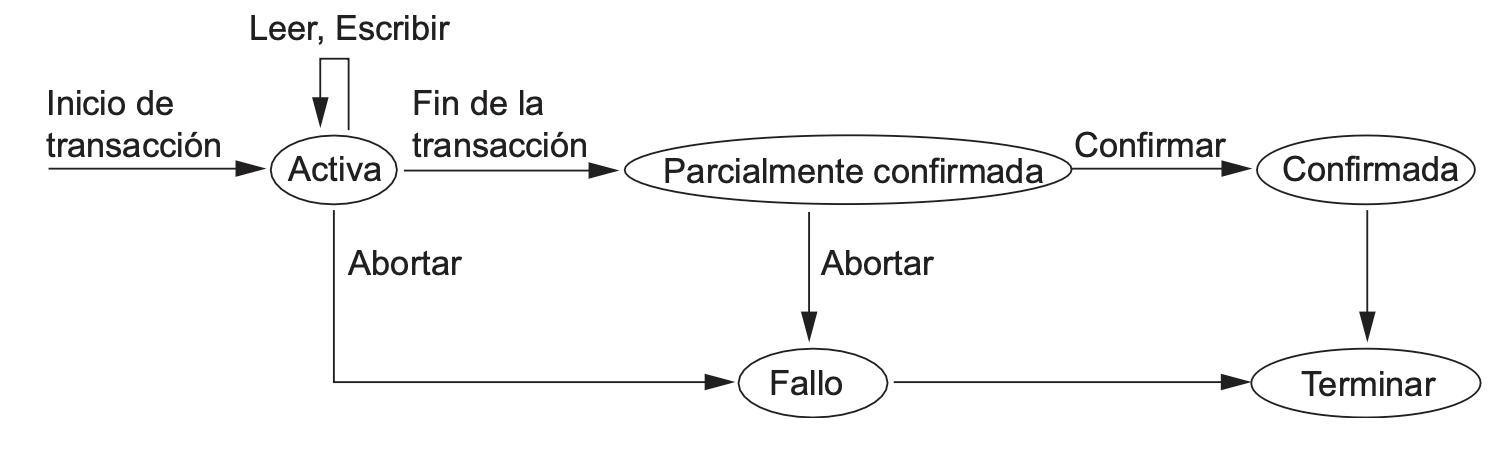
\includegraphics[scale=0.3]{img/transacciones.png}
 \end{figure}
 No-SQL
 \begin{itemize}
\item levelDB, rocksDB \dots
 \end{itemize}
}


%Las transacciones deben poseer varias propiedades, a menudo denominadas propiedades ACID, que deben ser implementadas por el control de la concurrencia y los métodos de recuperación del DBMS. Las propiedades ACID son las siguientes:
% Atomicidad. Una transacción es una unidad atómica de procesamiento; o se ejecuta en su totalidad o no se ejecuta en absoluto.
% Conservación de la consistencia. Una transacción está conservando la consistencia si su ejecución completa lleva a la base de datos de un estado consistente a otro.
% Aislamiento. Una transacción debe aparecer como si estuviera ejecutándose de forma aislada a las demás. Es decir, la ejecución de una transacción no debe interferir con la ejecución de ninguna otra transacción simultánea.
% Durabilidad. Los cambios aplicados a la base de datos por una transacción confirmada deben persis- tir en la base de datos. Estos cambios no deben perderse por culpa de un fallo.

  \end{frame}
  
  \begin{frame}{Evaluaciones}
  \begin{outline}
  	
  	\1 Controles (85\%):
	\2 Control 1:  Semana del 9 Mayo.
	\2 Control 2:  Semana del 13 Junio.
	\2 Control 3:  Semana del 11 Julio.
	\uncover<2->{
	\1 Tareas (15\%):
	\2 Tarea 1: Semana del 9 Mayo.
	\2 Tarea 2: Semana del 6 Junio. }
  \end{outline}
  \end{frame}
  
  \begin{frame}{Condiciones y Políticas de Evaluación}
  \small
  \begin{outline}
   \1 El promedio de actividades complementarias se considerará como un cuarto control (control IV) y tendrá una ponderación de 15\%. El promedio de controles I,II,III y IV con sus respectivas ponderaciones corresponderán a la nota final del curso. El curso será aprobado con una nota promedio igual o superior a 4,0.
    
 \uncover<2->{   \1 Estudiantes que se ausenten a un control tendrán la oportunidad de recuperarlo durante el periodo correspondiente al final del semestre. El control recuperativo es de carácter \textbf{acumulativo}, por lo tanto, contendrá contenido de las cuatro unidades del curso. Adicionalmente, alumnos que quieran remplazar una calificación en un control o actividades complementarias, también podrán rendir el control recuperativo.}
    
   \uncover<3->{ \1 Un/a estudiante que cometa plagio sobtendrá un 1,0 en la evaluación y el caso será informado a Escuela de Ingeniería.}
\end{outline}

  \end{frame}
  
  \begin{frame}{Materiales}
  \begin{outline}
  \1 Repositorio GitHub -- \url{https://github.com/adigenova/uohdb}
  \2 Clases
  \2 Notebooks para ejecutar en GoogleColab
  \uncover<2->{ \1 Ucampus -- \url{https://ucampus.uoh.cl/uoh/2022/1/COM3101}
  \2 Comunicación (Consultas, noticias, evaluaciones)
  \2 Planificacion }
 \uncover<3->{  \1 Bibliografía 
  \2 Ramez A. Elmasri, Shamkant B. Navathe, Fundamentos de Sistemas de Bases de Datos, 5a Edic., Addison Wesley. 2007 (Capitulo 1)
  \2 Molinaro, Anthony. SQL Cookbook. O’Reilly Media. (2009). }
  \end{outline}
  \end{frame} 
  
  \begin{frame}{Resultados de Aprendizaje}
  	\begin{outline}
		\1 Diseñar diagramas de Entidad/Relacional para satisfacer las necesidades de un problema enunciado.
		 \uncover<2->{ \1  Realizar a partir de un diagrama Entidad/Relación un diseño relacional.}
		 \uncover<3->{ \1 Normalizar un diseño relacional de bases de datos. }
		 \uncover<4->{ \1 Formular consultas de distinto tipo en SQL.}
		 \uncover<5->{ \1 Reconocer la noción de transacción y operar el sistema de recuperación de un sistema de administración de bases de datos.}
		 \uncover<6->{ \1 Conocer sistemas de bases de datos no relacionales.}
	\end{outline}
  \end{frame}
  
  \begin{frame}{Resumen}


A recordar

  \begin{outline}
  	\1 Que es una base de datos?
	\1 Cuales son las ventajas con respecto a una solución basada en archivos?
	\1 Que es un motor de bases de datos y cuales son sus principales funciones?
	\1 Que es SQL?
	\1 Para que sirve un esquema de bases de datos?
	\1 \dots
  \end{outline}
  
  Trabajo sugerido: \\
  Comenzar a interiorizarse con la plataforma \href{https://colab.research.google.com/}{GoogleColab}. \\
  Lectura opcional: \\
  Capitulo 1: Fundamentos de bases de datos.\\
  
  
  \end{frame}
  
  
    \begin{frame}{Consultas?}
    \centering 
    Consultas o comentarios?\\
    Muchas Gracias.
    
    \end{frame}

  
\end{document}